\documentclass{article}

\usepackage{amsmath}
\usepackage{amsthm}
\usepackage{graphicx}


\newtheorem{algorithm}{Algorithm}
\setlength\parindent{0pt}

\title{Group Assignment 1}
\author{Chance Zibolski, Dean Johnson}

\begin{document}
\maketitle

\section*{Problem}
Given an array of small integers $a[1,\ldots,n]$ (that contains a least one
positive integer), compute
\begin{eqnarray*}
  \label{MaxSubArray}
  \max_{i \leq j}\sum_{k=i}^{j}a[k]
\end{eqnarray*}


\begin{algorithm}
\textbf{Enumeration}: Loop over each pair of indices $ i \leq j $ and
compute the sum $\sum_{k=i}^{j}a[k]$
\end{algorithm}

\section*{Psuedocode}

\begin{verbatim}
MaxSubArray(a[1, ..., n])
  max_sum = 0
  sum = 0
  for i = 1, ..., n
    for j = i, ..., n
      for k = i, ..., j
        sum = sum + a[k]
      if sum > max_sum
        max_sum = sum
  return max_sum
\end{verbatim}

\section*{Run-time analysis}

\subsection*{Number of operations}
\begin{eqnarray*}
  \sum_{i=1}^{n}\sum_{j=i}^{n}\sum_{k=i}^{j}a[k]
\end{eqnarray*}

\subsection*{Asymptotic bounds}
\begin{eqnarray*}
    (\mathcal{O}(n^2) \times (\mathcal{O}(n) \text{time to compute each sum})) = \mathcal{O}(n^3)
\end{eqnarray*}

\begin{algorithm}
\textbf{Better Enumeration}: Notice that in the previous algorithm,  the
same sum is computed many times.  In particular, notice that
$\sum_{k=i}^{j}a[k]$ can be computed from $\sum_{k=i}^{j-1}a[k]$ in
$\mathcal{O}(1)$ time, rather than starting from scratch. Write a new version
of the first algorithm that takes advantage of this observation.
\end{algorithm}

\section*{Psuedocode}

\begin{verbatim}
MaxSubArray(a[1, ..., n])
  max_sum = 0
  for i = 1, ..., n
    sum = 0
    for j = i, ..., n
      sum = sum + a[j]
      if sum > max_sum
        max_sum = sum
  return max_sum
\end{verbatim}

\section*{Run-time analysis}

\subsection*{Number of operations}
\begin{eqnarray*}
  \sum_{i=1}^{n}\sum_{j=i}^{n}a[j]
\end{eqnarray*}

\subsection*{Asymptotic bounds}
\begin{eqnarray*}
    ((\mathcal{O}(n) \text{i-iterations}) \times
    (\mathcal{O}(n) \text{j-iterations}) \times
    (\mathcal{O}(n) \text{time to update sum}) ) = \mathcal{O}(n^2)
\end{eqnarray*}


\begin{algorithm}
\textbf{Dynamic Programming}: Your dynamic programming algorithm should be
based on the following idea:

\begin{itemize}
\item The maximum subarray either uses the last element in the input array,
or it doesn't.
\end{itemize}

Describe the solution to the maximum subarray problem recursively and
mathematically based on the above idea.
\end{algorithm}

\section*{Recursive Formula}

\[
  MaxSubArray(a[1, \ldots, n]) =
  \begin{cases}
      MaxSubArray\left(a[1, \ldots, \frac{n}{2}]\right)\\
      MaxSubArray\left(a[\frac{n}{2}, \ldots, n]\right)\\
      MaxSuffix\left(a[1, \ldots, \frac{n}{2}]\right) +
      MaxPrefix\left(a[\frac{n}{2}, \ldots, n]\right)\\
  \end{cases}
\]

\begin{verbatim}
MaxSuffix(a[low, ..., mid])
  max = 0
  sum = 0
  for i = mid, ..., low
    sum = sum + a[i]
    if sum > max
      max = sum
  return max

MaxPrefix(a[mid, ..., high])
  max = 0
  sum = 0
  for i = mid, ..., high
    sum = sum + a[i]
    if sum > max
      max = sum
  return max
\end{verbatim}

\section*{Psuedocode}

\begin{verbatim}
MaxSubArray(a[1, ..., n])
  max = 0
  sum = 0
  for i = 1, ..., n
    sum = sum + a[i]
    if sum < 0
      sum = 0
    if sum > max
      max = sum
  return max
\end{verbatim}

\section*{Run-time analysis}

\subsection*{Number of operations}
\begin{eqnarray*}
  \sum_{i=1}^{n}a[i]
\end{eqnarray*}

\subsection*{Asymptotic bounds}
\begin{eqnarray*}
    (\mathcal{O}(n) \text{i-iterations}) \times
    (\mathcal{O}(c) \text{to compute sum}) = \mathcal{O}(n)
\end{eqnarray*}

\section{Graphs}

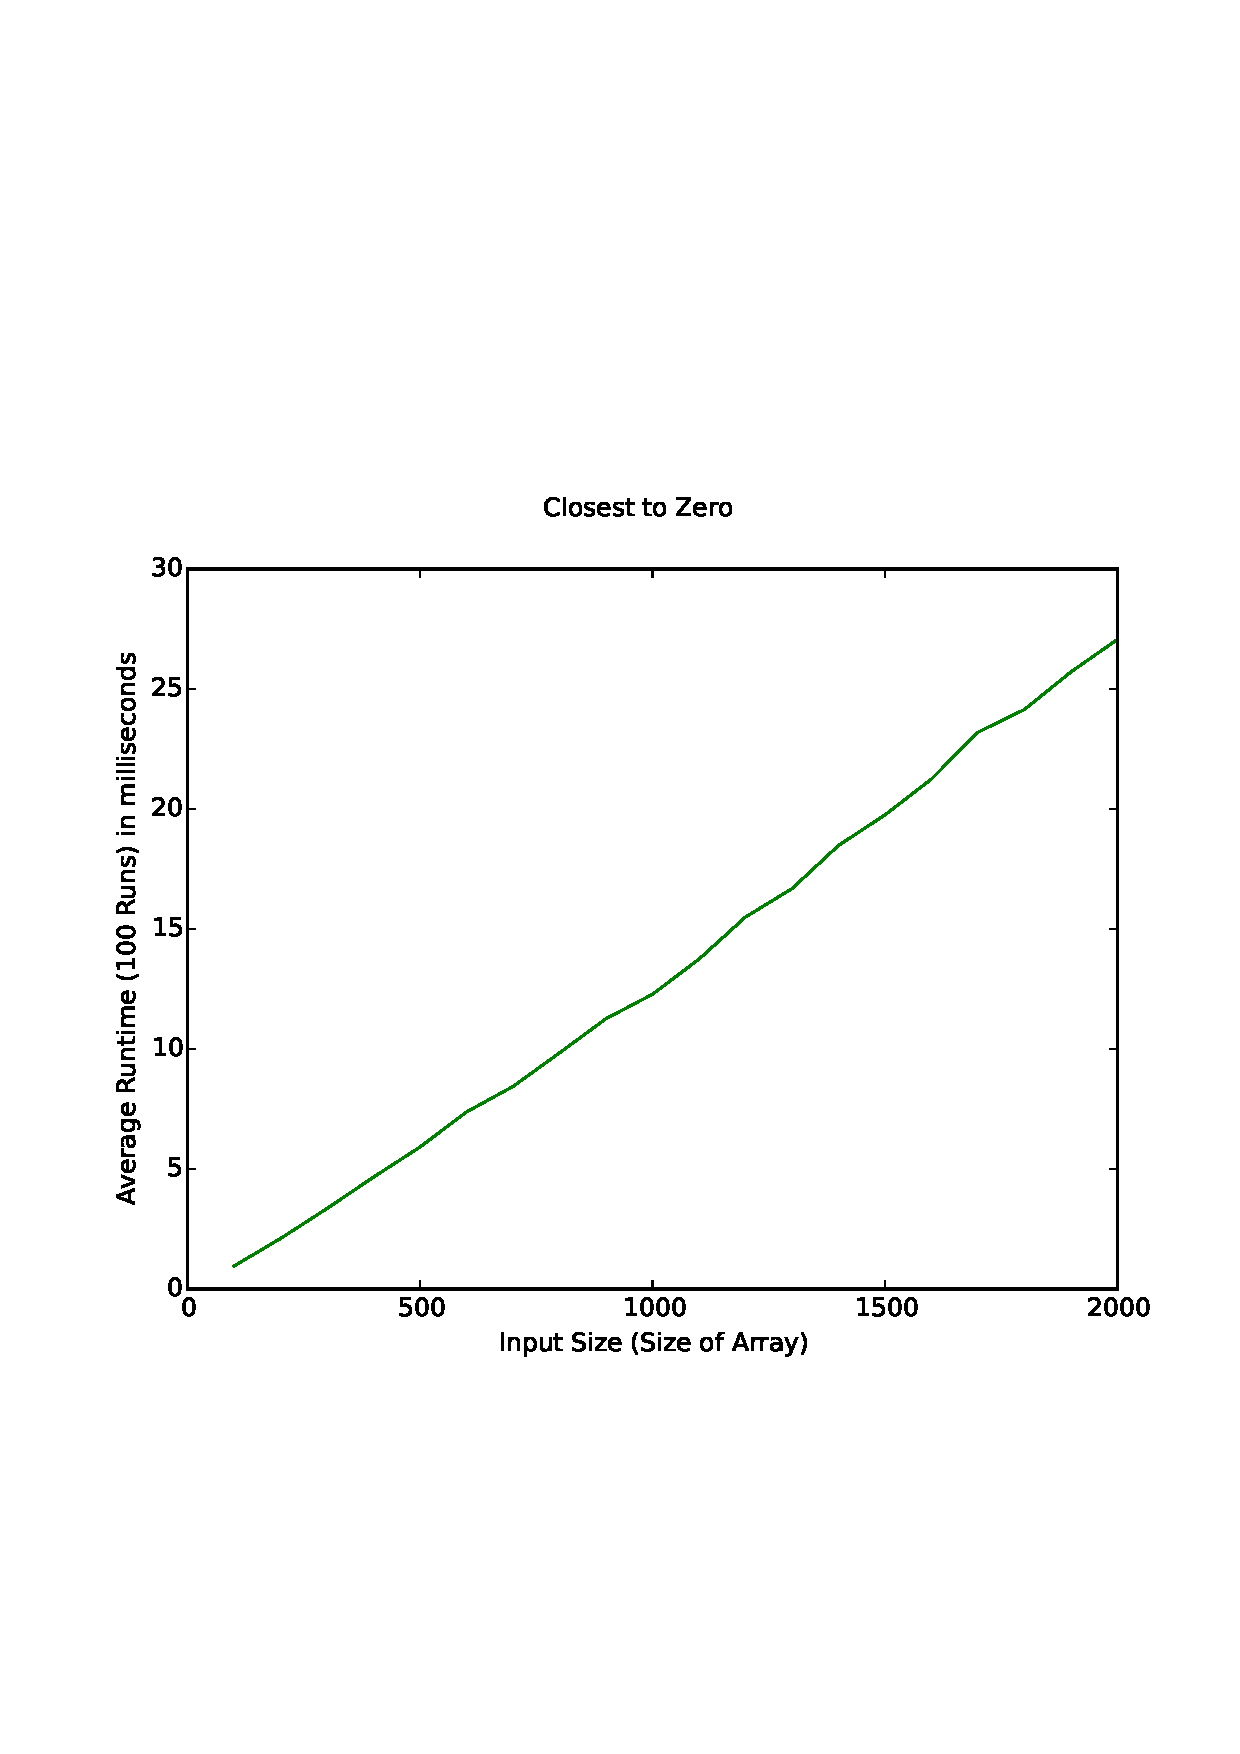
\includegraphics[width=\textwidth]{timings}

\subsubsection*{Slope comparision}

During our experiments we obtained the following slopes for our algorithms:

\begin{itemize}
\item Algorithm 1: 2.6283
\item Algorithm 2: 1.9803
\item Algorithm 3: 0.9920
\end{itemize}

This would give us the following runtime complexity for each algorithm:

\begin{itemize}
    \item Algorithm 1: $\mathcal{\theta}(n^{2.6283})$
    \item Algorithm 2: $\mathcal{\theta}(n^{1.9803})$
    \item Algorithm 3: $\mathcal{\theta}(n^{0.9920})$
\end{itemize}

These values are extremely close to what we would have expected. The only
algorithm which had a value that was not completely accurate was algorithm 1.
This can be partially attributed to the fact that algorithm 1 was the only
algorithm which was not tested with sets greater than 900 elements.

\end{document}
